% Created 2021-05-13 Thu 07:34
% Intended LaTeX compiler: pdflatex
\documentclass[presentation]{beamer}
\usepackage[utf8]{inputenc}
\usepackage[T1]{fontenc}
\usepackage{graphicx}
\usepackage{grffile}
\usepackage{longtable}
\usepackage{wrapfig}
\usepackage{rotating}
\usepackage[normalem]{ulem}
\usepackage{amsmath}
\usepackage{textcomp}
\usepackage{amssymb}
\usepackage{capt-of}
\usepackage{hyperref}
\RequirePackage{fancyvrb}
\DefineVerbatimEnvironment{verbatim}{Verbatim}{fontsize=\scriptsize}
\usetheme{metropolis}
\usecolortheme{}
\usefonttheme{}
\useinnertheme{}
\useoutertheme{}
\author{Petru Rebeja, Marius Apetrii}
\date{13 Mai 2021}
\title{Tehnici Avansate de Programare}
\subtitle{\texttt{TPL}, \texttt{middleware} şi securitatea în ASP.NET Core MVC}
\institute[UAIC]{Facultatea de Matematică\\Universitatea Alexandru Ioan Cuza, Iași}
\hypersetup{
 pdfauthor={Petru Rebeja, Marius Apetrii},
 pdftitle={Tehnici Avansate de Programare},
 pdfkeywords={},
 pdfsubject={},
 pdfcreator={Emacs 26.3 (Org mode 9.4.4)},
 pdflang={Romanian}}
\begin{document}

\maketitle
\section{Introducere}
\label{sec:orgadd0e02}
\begin{frame}[label={sec:org0733dad},fragile]{Recapitulare}
 \pause
\begin{itemize}
\item \alert{MVC} este un şablon de proiectare utilizat pentru a decupla interfaţa grafică (\texttt{view}), datele (\texttt{model}) şi logica aplicaţiei (\texttt{controller}).
\end{itemize}
\pause
\begin{itemize}
\item \alert{ASP.NET Core MVC} este o platformă \texttt{open-source} care permite dezvoltarea de aplicaţii Web pe baza convenţiilor asociate şablonului \texttt{MVC}.
\end{itemize}
\end{frame}
\begin{frame}[label={sec:org491c8d4},fragile]{Agenda}
 \begin{itemize}
\item Task Parallel Library
\item Middleware
\item Securitatea în \texttt{ASP.NET Core MVC}
\end{itemize}
\end{frame}
\section{\texttt{Task Parallel Library}}
\label{sec:org22792d6}
\begin{frame}[label={sec:org5de85cf}]{Execuţie sincronă vs asincronă}
Exemplu: Încărcarea unei pagini web de către server.
\vskip 0.1in
Utilizatorii A  şi B deschid pagina web din navigatorul web. Pentru a încărca datele serverul trece prin următorii paşi.
\end{frame}
\begin{frame}[label={sec:orgd9fd7d4}]{Execuţie sincronă}
\begin{enumerate}
\item Trimite interogare la baza de date pentru A
\item Aşteaptă răspunsul
\item Primeşte răspuns de la baza de date pentru A
\item Generează HTML-ul
\item Trimite răspuns lui A
\item Trimite interogarea la baza de date pentru B
\item Aşteaptă răspunsul
\item Primeşte răspuns la interogarea pentru B
\item Generează HTML-ul pentru B
\item Trimite răspuns lui B
\end{enumerate}
\end{frame}
\begin{frame}[label={sec:orga69a0ec}]{Execuţie asincronă}
\begin{enumerate}
\item Trimite interogare la baza de date pentru utilizatorul A
\item Trimite interogare la baza de date pentru utilizatorul B
\item Primeşte răspuns la interogarea pentru A
\item Generează HTML-ul pentru A
\item Trimite răspuns lui A
\item Primeşte răspuns la interogarea pentru B
\item Generează HTML-ul pentru B
\item Trimite răspuns lui B
\end{enumerate}
\end{frame}
\begin{frame}[label={sec:org3978cc1},fragile]{Ce este \texttt{TPL}}
 \begin{block}{\texttt{Task Parallel Library}\footnote{\url{https://docs.microsoft.com/en-us/dotnet/standard/parallel-programming/task-parallel-library-tpl}}}
\vskip 0.1in
O mulţime de tipuri şi funcţii pentru a simplifica integrarea execuţiei paralele şi concurente într-o aplicaţie.
\end{block}
\end{frame}
\begin{frame}[label={sec:org49c72ab},fragile]{Beneficiile \texttt{TPL}\footnote{\url{https://docs.microsoft.com/en-us/dotnet/standard/parallel-programming/task-parallel-library-tpl}}}
 \begin{itemize}
\item Utilizarea eficientă a procesoarelor.
\item Distribuie eficient munca între firele de execuţie.
\item Gestionează automat detalii precum:
\begin{itemize}
\item Alocarea timpului de procesor,
\item Tranziţia între stări etc.
\end{itemize}
\item Oferă suport pentru anulare.
\item Reduce codul de umplutură.
\end{itemize}
\end{frame}
\begin{frame}[label={sec:orga198b15}]{Imaginea de ansamblu\footnote{\url{http://www.albahari.com/threading/part5.aspx}}}
\begin{center}
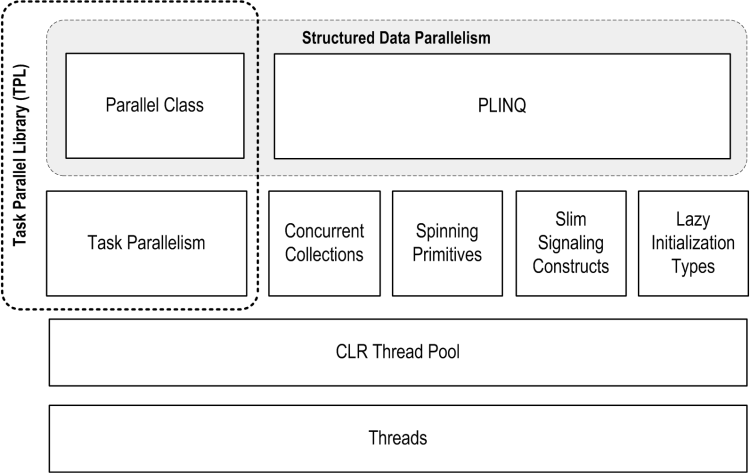
\includegraphics[height=.7\textheight]{img/tpl.png}
\end{center}
\end{frame}
\begin{frame}[label={sec:orgf6d4492},fragile]{Ce este un \texttt{Task}}
 \begin{itemize}
\item Unitatea de bază din \texttt{TPL}.
\item Reprezintă o operaţie care este executată asincron\footnote{\url{https://docs.microsoft.com/en-us/dotnet/api/system.threading.tasks.task}} şi poate întoarce un rezultat.
\end{itemize}
\end{frame}
\begin{frame}[label={sec:org713477f},fragile]{\texttt{Task} vs \texttt{Thread}}
 \begin{itemize}
\item Un fir de execuţie poate executa mai multe \texttt{Taskuri}.
\item Un \texttt{Task} poate întoarce un rezultat (prin proprietatea \texttt{Result}); un fir de execuţie nu.
\end{itemize}
\end{frame}
\begin{frame}[label={sec:orgb724d44},fragile]{\texttt{Task} vs \texttt{Thread}\footnote{Diagrama este simplificată la un singur fir de execuţie per nucleu (core) .}}
 \begin{center}
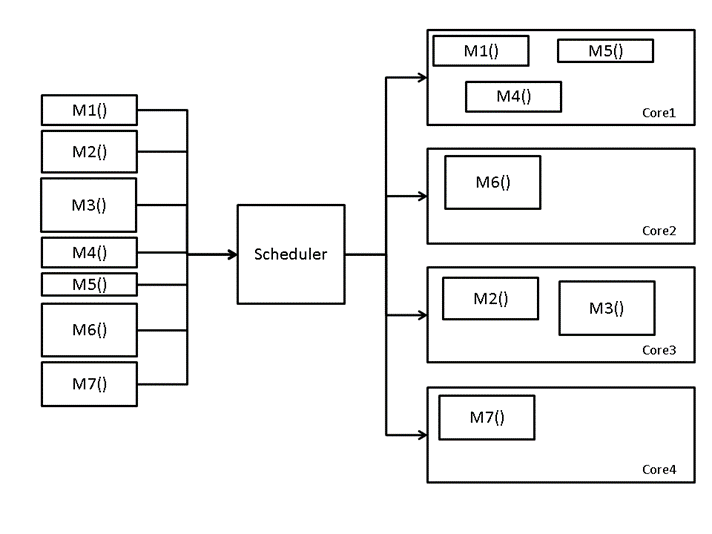
\includegraphics[height=.8\textheight]{img/task-parallelism.png}
\end{center}
\end{frame}
\begin{frame}[label={sec:org6ccaa45},fragile]{Async \& await}
 \begin{itemize}
\item \texttt{async} este aplicat în declaraţia metodei pentru a semnala că metoda se execută asincron.
\item Metodele declarate cu \texttt{async} trebuie să întoarcă un \texttt{Task} sau un \texttt{Task<T>}.
\item \texttt{await} este un operator care suspendă execuţia metodei marcată cu \texttt{await} până la terminarea execuţiei operandului. Apoi metoda îşi reia execuţia.
\end{itemize}
\end{frame}
\section{\texttt{Middleware}}
\label{sec:orgcd3efb6}
\begin{frame}[label={sec:orgeb771c5},fragile]{Ce este \texttt{middleware}?}
 \begin{block}{\texttt{Middleware}}
\vskip 0.1in
Componente software asamblate într-un sistem pentru a defini un flux de lucru care să proceseze interogările venite de la utilizatori şi răspunsurile la aceste interogări\footnote{\url{https://docs.microsoft.com/en-us/aspnet/core/fundamentals/middleware/}}.
\end{block}
\end{frame}
\begin{frame}[label={sec:orgc61e266},fragile]{\texttt{Middleware}\footnote{\url{https://andrewlock.net/asp-net-core-in-action-what-is-middleware/}}}
 \begin{center}
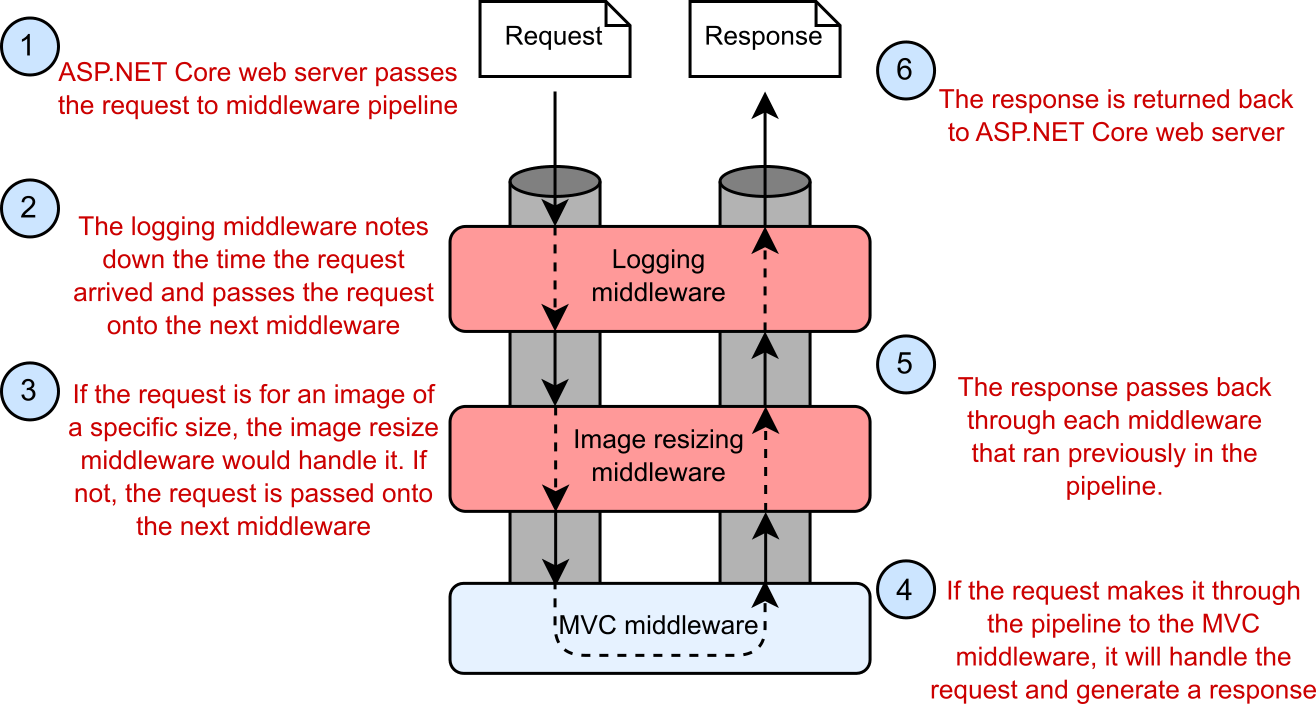
\includegraphics[width=\textwidth]{img/middleware.png}
\end{center}
\end{frame}
\section{Securitatea în \texttt{ASP.NET Core MVC}}
\label{sec:org91e4446}
\begin{frame}[label={sec:org4622a4c}]{Autentificare}
\begin{block}{Autentificare}
\vskip 0.1in
Procesul de preluare a datelor care atestă identitatea unui utilizator şi verificarea acestora.
\end{block}
\end{frame}
\begin{frame}[label={sec:org8ebc3aa}]{Autorizare}
\begin{block}{Autorizare}
\vskip 0.1in
Procesul de verificare a drepturilor de acces a  unui utilizator în vederea accesării unei anumite resurse.
\end{block}
\end{frame}
\begin{frame}[label={sec:org1c925bc}]{ASP.NET Core Identity}
\begin{itemize}
\item Bibliotecă pentru implementarea autentificării.
\item Gestionează utilizatori, parole, roluri ş.a.
\end{itemize}
\end{frame}
\begin{frame}[label={sec:org5241dc7}]{Componente\footnote{\url{https://docs.microsoft.com/en-us/aspnet/core/security/authentication/identity-custom-storage-providers}}}
\begin{center}
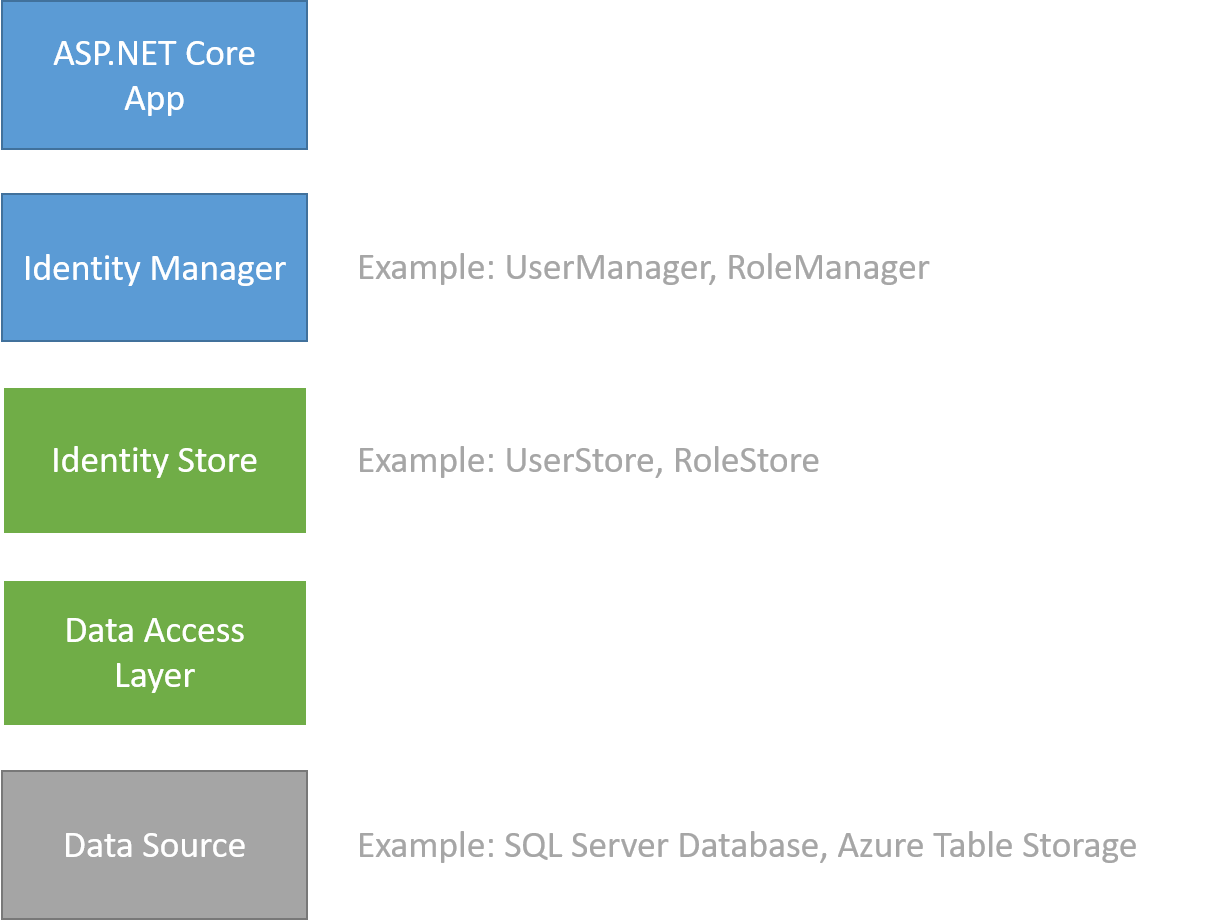
\includegraphics[height=.7\textheight]{img/identity-architecture-diagram.png}
\end{center}
\end{frame}
\begin{frame}[label={sec:org6e64615},fragile]{Autorizarea}
 \begin{itemize}
\item Se face prin adnotarea controllerului sau metodelor din controller cu atributul \texttt{AuthorizeAttribute}.
\item Poate fi de mai multe feluri.
\end{itemize}
\end{frame}
\begin{frame}[label={sec:org38c91ed},fragile]{Tipuri de autorizare\footnote{\url{https://docs.microsoft.com/en-us/aspnet/core/security/authorization/introduction}}}
 \begin{itemize}
\item Simplă: \texttt{[Authorize]}
\item Pe bază de roluri: \texttt{[Authorize(Roles="Admin;Manager")]}
\item Pe bază de reguli: \texttt{[Authorize(Policy="EmployeeOnly")]}
\end{itemize}
\end{frame}
\begin{frame}[label={sec:org2314a3e}]{Fluxul de lucru pentru autentificare şi autorizare\footnote{\url{https://andrewlock.net/asp-net-core-in-action-what-is-middleware/}}}
\begin{center}
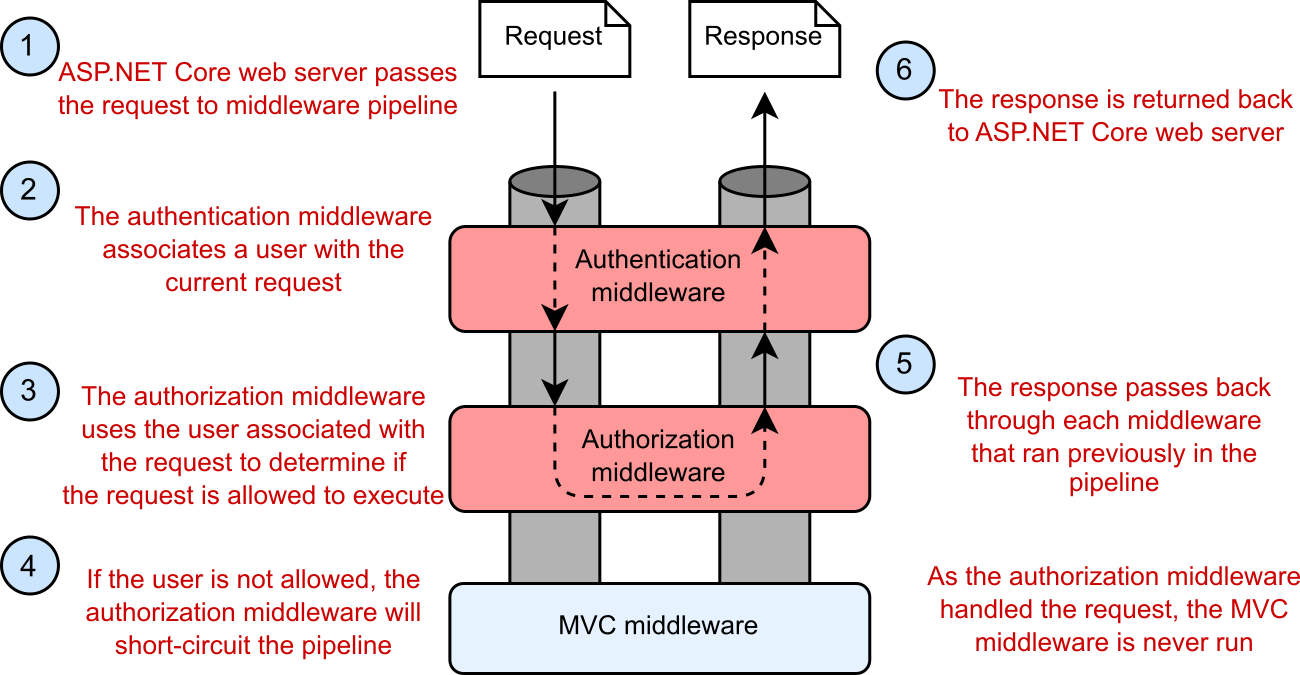
\includegraphics[width=\textwidth]{img/auth.png}
\end{center}
\end{frame}
\section{Încheiere}
\label{sec:org7e4fa60}
\begin{frame}[label={sec:org6ae7c3a},fragile]{Recapitulare}
 \begin{itemize}
\item \texttt{TPL} simplifică integrarea execuţiei paralele şi asincrone în aplicaţie lăsând în grija sistemului detaliile de nivel inferior a.î. programatorul să se poată concentra asupra logicii aplicaţiei.
\item \texttt{Middleware} sunt componentele care fac parte din linia de procesare a interogărilor şi răspunsurilor la interogări.
\item Două componente de acest fel sunt middleware pentru autentificare şi autorizare care se ocupă de atestarea identităţii utilizatorului şi respectiv verificarea drepturilor de acces.
\item Putem folosi \texttt{ASP.NET Core Identity} pentru a implementa autentificarea.
\item Autorizarea se face cu ajutorul \texttt{AuthorizeAttribute}.
\end{itemize}
\end{frame}
\begin{frame}[label={sec:org6fee171}]{Vă mulțumesc!}
\begin{center}
Mulțumesc pentru atenție!
\end{center}
\end{frame}
\end{document}